
\definecolor{deepskyblue}{RGB}{0,191,255}
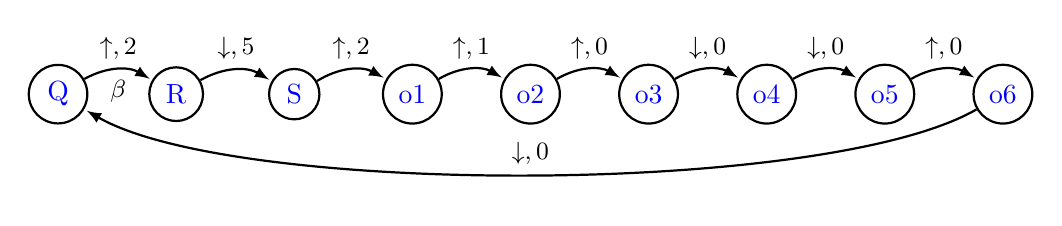
\begin{tikzpicture}[->,>=latex,shorten >=1pt,auto,node distance=1.5cm,
      thick,main node/.style={circle,draw}]
 \node[main node, fill=white, text=blue] (Q)  {Q};
 \node[main node, fill=white, text=blue] (R) [right of=Q] {R};
 \node[main node, fill=white, text=blue] (S) [right of=R] {S};
 \node[main node, fill=white, text=blue] (o1) [right of=S] {o1};
 \node[main node, fill=white, text=blue] (o2) [right of=o1] {o2};
 \node[main node, fill=white, text=blue] (o3) [right of=o2] {o3};
 \node[main node, fill=white, text=blue] (o4) [right of=o3] {o4};
 \node[main node, fill=white, text=blue] (o5) [right of=o4] {o5};
 \node[main node, fill=white, text=blue] (o6) [right of=o5] {o6};
 
\path[every node/.style={font=\sffamily\small}]
 (Q) edge [bend left] node [above] {$\uparrow, 2$} node [below] {$\beta$} (R)
 (R) edge [bend left] node [above] {$\downarrow, 5$} node [below] {} (S)
 (S) edge [bend left] node [above] {$\uparrow, 2$} node [below] {} (o1)
 (o1) edge [bend left] node [above] {$\uparrow, 1$} node [below] {} (o2)
 (o2) edge [bend left] node [above] {$\uparrow, 0$} node [below] {} (o3)
 (o3) edge [bend left] node [above] {$\downarrow, 0$} node [below] {} (o4)
 (o4) edge [bend left] node [above] {$\downarrow, 0$} node [below] {} (o5)
 (o5) edge [bend left] node [above] {$\uparrow, 0$} node [below] {} (o6)
 (o6) edge [bend left, looseness=0.5] node [above] {$\downarrow, 0$} node [below] {} (Q)
 ;
\end{tikzpicture}
